% !TeX root = er.tex

\chapter{Mapping-Based Navigation}\label{ch.map-based}
\index{navigation!map-based}

\abstract*{Given a map and a target position, a robot must perform path planning in order to determine the best route from its current position to the target position. Three algorithms for path planning are presented: Dijkstra's shortest path algorithm for a grid of cells, an algorithm for continuous maps and the A$\!^{*}$ algorithm, an improvement of Dijkstra's algorithm that uses heuristic functions. The chapter concludes with a description of the integration of path planning with obstacle avoidance.}

Now that we have a map, whether supplied by the user or discovered by the robot, we can discuss \emph{path planning}, a higher-level algorithm. Consider a robot used in a hospital for transporting medications and other supplies from storage areas to the doctors and nurses. Given one of these tasks, what is the best way of going from point A to point B. There may be multiple ways of moving through the corridors to get to the goal, but there may also be short paths that the robot is not allowed to take, for example, paths that go through corridors near the operating rooms.

We present three algorithms for planning the shortest path from a starting position \p{S} to a goal position \p{G}, assuming that we have a map of the area that indicates the positions of obstacles in the area. Edsgar W. Dijkstra, one of the pioneers of computer science, proposed an algorithm for the shortest path problem. Section~\ref{s.dijkstra-grid} describes the algorithm for a grid map, while Sect.~\ref{s.dijkstra-continuous} describes the algorithm for a continuous map. The \astar{} algorithm, an improvement on Dijkstra's algorithm based upon heuristic methods, is presented in Sect.~\ref{s.astar}. Finally, Sect.~\ref{s.path-and-obstacle} discusses how to combine a high-level path planning algorithm with a low-level obstacle avoidance algorithm.

\section{Dijkstra's algorithm for a grid map}\label{s.dijkstra-grid}
\index{Dijkstra's algorithm}

Dijkstra described his algorithm for a discrete graph of nodes and edges. Here we describe it for a grid map of cells (Fig.~\ref{fig.dijkstra-grid}). Cell \p{S} is the starting cell of the robot and its task is to move to the goal cell \p{G}. Cells that contain obstacles are shown in black. The robot can sense and move to a \emph{neighbor} of the cell \p{c} it occupies. For simplicity, we specify that the neighbors of \p{c} are the four cells next to it horizontally and vertically, but not diagonally. Figure~\ref{fig.dijkstra-path} shows a shortest path from \p{S} to \p{G}:
\[
\begin{array}{ll}
(4,0) \rightarrow &(4,1)\rightarrow (3,1) \rightarrow (2,1) \rightarrow (2,2) \rightarrow \\
&(2,3) \rightarrow (3,3) \rightarrow (3,4) \rightarrow (3,5) \rightarrow (4,5)\,.
\end{array}
\]

\begin{figure}
\subfigures
\begin{minipage}{\textwidth}
\leftfigure[c]{
\begin{tikzpicture}[scale=.8]
\pic[scale=.8] at (0,0) {astar};
\end{tikzpicture}
}
\hspace{\fill}
\rightfigure[c]{
\begin{tikzpicture}[scale=.8]
\pic[scale=.8] at (0,0) {astar};
\begin{scope}[xshift=.5cm,yshift=.5cm]
\draw[->,thick,blue] (.2,0) -- (1,0);
\draw[->,thick,blue] (1,0) -- (1,1);
\draw[->,thick,blue] (1,1) -- (1,2);
\draw[->,thick,blue] (1,2) -- (2,2);
\draw[->,thick,blue] (2,2) -- (3,2);
\draw[->,thick,blue] (3,2) -- (3,1);
\draw[->,thick,blue] (3,1) -- (4,1);
\draw[->,thick,blue] (4,1) -- (5,1);
\draw[->,thick,blue] (5,1) -- (5,.2);
\end{scope}
\end{tikzpicture}
}
\leftcaption{Grid map for Dijkstra's algorithm}\label{fig.dijkstra-grid}\rightcaption{The shortest path found by Dijkstra's algorithm}\label{fig.dijkstra-path}
\end{minipage}
\end{figure}

Two versions of the algorithm are presented: The first is for grids where the cost of moving from one cell to one of its neighbors is constant. In the second version, each cell can have a different cost associated with moving to it, so the shortest path geometrically is not necessarily the shortest path when the costs are taken into account.

\subsection{Dijkstra's algorithm on a grid map with constant cost}
\index{Dijkstra's algorithm!grid map with constant cost}

Algorithm~\ref{alg.dijkstra-grid} is Dijkstra's algorithm for a grid map. The algorithm is demonstrated on the $5\times 6$ cell grid map in Fig.~\ref{fig.dijkstra-simple}. There are three obstacles represented by the black cells.

\begin{figure}
\begin{alg}{Dijkstra's algorithm on a grid map}{dijkstra-grid}
&\idv{}integer n \ass 0&// Distance from start\\
&\idv{}cell array grid \ass all unmarked&// Grid map\\
&\idv{}cell list path \ass empty&// Shortest path\\
&\idv{}cell current&// Current cell in path\\
&\idv{}cell c&// Index over cells\\
&\idv{}cell S \ass $\cdots$&// Source cell\\
&\idv{}cell G \ass $\cdots$&// Goal cell\\
\hline
\stl{}&mark S with n&\\
\stl{}&while G is unmarked&\\
\stl{}&\idc{}n \ass n $+$ 1&\\
\stl{}&\idc{}for each unmarked cell c in grid&\\
\stl{}&\idc{}\idc{}\idc{}next to a marked cell&\\
\stl{}&\idc{}\idc{}mark c with n&\\
\stl{}&current \ass G&\\
\stl{}&append current to path&\\
\stl{}&while S not in path&\\
\stl{}&\idc{}append lowest marked neighbor c&\\
\stl{}&\idc{}\idc{}of current to path&\\
\stl{}&\idc{}current \ass c&\\
\end{alg}
\end{figure}


\begin{figure}
\subfigures
\begin{minipage}{\textwidth}
\leftfigure[c]{
\begin{tikzpicture}[scale=.8]
\pic[scale=.8] at (0,0) {astar};
\end{tikzpicture}
}
\hspace{\fill}
\rightfigure[c]{
\begin{tikzpicture}[scale=.8]
\pic[scale=.8] at (0,0) {astar};
\foreach \x/\y/\n in {0/0/0, 1/0/1, 0/1/1, 1/1/2, 0/2/2}
  \node at (\x+.2,\y+.8) {\p{\n}};
\end{tikzpicture}
}
\leftcaption{Grid map for Dijkstra's algorithm}\label{fig.dijkstra-simple}
\rightcaption{The first two iterations of Dijkstra's algorithm}\label{fig.dijkstra-simple-2}
\end{minipage}
\end{figure}

The algorithm incrementally marks each cell \p{c} with the number of steps needed to reach \p{c} from the start cell \p{S}. In the figures, the step count is shown as a number in the upper left hand corner of a cell. Initially, mark cell \p{S} with $0$ since no steps are needed to reach \p{S} from \p{S}. Now, mark every neighbor of \p{S} with $1$ since they are one step away from \p{S}; then mark every neighbor of a cell marked $1$ with $2$. Figure~\ref{fig.dijkstra-simple-2} shows the grid map after these two iterations of the algorithm.

\begin{figure}
\subfigures
\begin{minipage}{\textwidth}
\leftfigure[c]{
\begin{tikzpicture}[scale=.8]
\pic[scale=.8] at (0,0) {astar};
\foreach \x/\y/\n in {0/0/0, 1/0/1, 0/1/1, 1/1/2, 0/2/2, 0/3/3, 1/2/3, 0/4/4, 1/3/4, 2/2/4, 3/2/5, 1/4/5}
  \node at (\x+.2,\y+.8) {\p{\n}};
\end{tikzpicture}
}
\hspace{\fill}
\rightfigure[c]{
\begin{tikzpicture}[scale=.8]
\foreach \x/\y in {0/0, 1/0, 1/1, 1/2, 2/2, 3/2, 3/1, 4/1, 5/1, 5/0}
  \draw[fill,lightgray] (\x,\y) rectangle +(1,1);
\pic[scale=.8] at (0,0) {astar};
\foreach \x/\y/\n in {0/0/0, 1/0/1, 0/1/1, 1/1/2, 0/2/2, 0/3/3, 1/2/3, 0/4/4, 1/3/4, 2/2/4, 3/2/5, 1/4/5, 3/3/6, 3/1/6, 3/4/7, 3/0/7, 4/1/7, 4/3/7, 4/0/8, 5/3/8, 4/4/8, 5/1/8, 5/4/9, 5/0/9}
  \node at (\x+.2,\y+.8) {\p{\n}};
\end{tikzpicture}
}
\leftcaption{After five iterations of Dijkstra's algorithm\label{fig.dijkstra-simple-5}}
\rightcaption{The final grid map with the shortest path marked\label{fig.dijkstra-simple-9}}
\end{minipage}
\end{figure}

The algorithm continues iteratively: if a cell is marked $n$, its unmarked neighbors are marked with $n+1$. When \p{G} is finally marked, we know that the shortest distance from \p{S} to \p{G} is $n$. Fig.~\ref{fig.dijkstra-simple-5} shows the grid map after five iterations and Fig.~\ref{fig.dijkstra-simple-9} shows the final grid map after nine iterations when the goal cell has been reached.

It is now easy to find a shortest path by working backwards from the goal cell \p{G}. In Fig.~\ref{fig.dijkstra-simple-9} a shortest path consists of the cells that are colored gray. Starting with the goal cell at coordinate $(4,5)$, the previous cell must be either $(4,4)$ or $(3,5)$ since they are eight steps away from the start. (This shows that there is more than one shortest path.) We arbitrarily choose $(3,5)$. From each selected cell marked $n$, we choose a cell marked $n-1$ until the cell \p{S} marked $0$ is selected. The list of the selected cells is:
\[
(4,5),\, (3,5),\, (3,4),\, (3,3),\, (2,3),\, (2,2),\, (2,1),\, (3,1),\, (4,1),\, (4,0)\,.
\]
By reversing the list, the shortest path from \p{S} to \p{G} is obtained. Check that this is the same path we found intuitively (Fig.~\ref{fig.dijkstra-path}).

\medskip

\noindent\textbf{Example} Figure~\ref{fig.dijkstra} shows how Dijkstra's algorithm works on a more complicated example. The grid map has $16\times 16$ cells and the goal cell \p{G} is enclosed within an obstacle and difficult to reach. The upper left diagram shows the grid map after three iterations and the upper right diagram shows the map after $19$ iterations. The algorithm now proceeds by exploring cells around both sides of the obstacle. Finally, in the lower left diagram, \p{G} is found after $25$ iterations, and the shortest path is indicated in gray in the lower right diagram. We see that the algorithm is not very efficient for this map: although the shortest path is only $25$ steps, the algorithm has explored $256-25=231$ cells!

\begin{figure}
\begin{center}
\includegraphics[width=.9\textwidth]{images/grid-plan.pdf}
\end{center}
\caption{Dijkstra's algorithm for path planning on a grid map. Four stages in the execution of the algorithm are shown starting in the upper left diagram.}\label{fig.dijkstra}
\end{figure}

\subsection{Dijkstra's algorithm with variable costs}
\index{Dijkstra's algorithm!grid map with variable cost}

Algorithm~\ref{alg.dijkstra-grid} and the example in Fig.~\ref{fig.dijkstra} assume that the cost of taking a step from one cell to the next is constant: line three of the algorithm adds $1$ to the cost for each neighbor. Dijkstra's algorithm can be modified to take into account a variable cost of each step. Suppose that an area in the environment is covered with sand and that it is more difficult for the robot to move through this area. In the algorithm, instead of adding $1$ to the cost for each neighboring cell, we can add $k$ to each neighboring sandy cell to reflect the additional cost.

\begin{figure}
\begin{center}
\includegraphics[width=.9\textwidth]{images/grid-plad-sand.pdf}
\end{center}
\caption{Dijkstra's algorithm with a variable cost per cell (left diagram, cost=$4$, right diagram, cost=$2$)}\label{fig.path-sand}
\end{figure}

The grid on the left of Fig.~\ref{fig.path-sand} has some cells marked with a diagonal line to indicate that they are covered with sand and that the cost of moving through them is $4$ and not $1$. The shortest path, marked in gray, has $17$ steps and also costs $17$ since it goes around the sand.

The shortest path depends on the cost assigned to each cell. The right diagram shows the shortest path if the cost of moving through a cell with sand is only $2$. The path is $12$ steps long although its cost is $14$ to take into account moving two steps through the sand.

\begin{framed}
\act{Dijkstra's algorithm on a grid map}{dijkstra-grid}
\begin{itemize}
\item Construct a grid map and apply Dijkstra's algorithm.
\item Modify the map to include cells with a variable cost and apply the algorithm.
\item Implement Dijkstra's algorithm.
\begin{itemize}
\item Create a grid on the floor.
\item Write a program that causes the robot to move from a known start cell to a known goal cell. Since the robot must store its current location, use this to create a map of the cells it has moved through.
\item Place some obstacles in the grid and enter them in the map of the robot.
\end{itemize}
\end{itemize}
\end{framed}


\section{Dijkstra's algorithm for a continuous map}\label{s.dijkstra-continuous}
\index{Dijkstra's algorithm!continuous map}

In a continuous map the area is an ordinary two-dimensional geometric plane. One approach to using Dijkstra's algorithm in a continuous map is to transform the map into a discrete graph by drawing vertical lines from the upper and lower edges of the environment to each corner of an obstacle. This divides the area into a finite number of segments, each of which can be represented as a node in a graph. The left diagram of Fig.~\ref{fig.map-graph-at} shows seven vertical lines that divide the map into ten segments which are shown in the graph in Fig.~\ref{fig.map-graph-ab}. The edges of the graph are defined by the adjacency relation of the segments. There is a directed edge from segment \p{A} to segment \p{B} if \p{A} and \p{B} share a common border. For example, there are edges from node $2$ to nodes $1$ and $3$ since the corresponding segments share an edge with segment $2$.

\begin{figure}
\begin{center}
\includegraphics[width=\textwidth]{images/plan-continuous2at.pdf}
\end{center}
\caption{Segmenting a continuous map by vertical lines and the path through the segments}\label{fig.map-graph-at}
\end{figure}

\begin{figure}
\begin{center}
\includegraphics[width=.8\textwidth]{images/plan-continuous2ab.pdf}
\end{center}
\caption{The graph constructed from the segmented continuous map}\label{fig.map-graph-ab}
\end{figure}

What is the shortest path between vertex $2$ representing the segment containing the starting point and vertex $10$ representing the segment containing the goal? The result of applying Dijkstra's algorithm is $\p{S} \rightarrow 2\rightarrow 3\rightarrow 6\rightarrow 9\rightarrow 10 \rightarrow \p{G}$. Although this is the shortest path in terms of the number of edges of the graph, it is not the shortest path in the environment. The reason is that we assigned constant cost to each edge, although the segments of the map have various size. 

Since each vertex represents a large segment of the environment, we need to know how moving from one vertex to another translates into moving from one segment to another. The right diagram in Fig.~\ref{fig.map-graph-at} shows one possibility: each segment is associated with its geometric center, indicated by the intersection of the dotted diagonal lines in the figure. The path in the environment associated with the path in the graph goes from the center of one segment to the center of the next segment, except that the start and goal positions are at their geometric locations. Although this method is reasonable without further knowledge of the environment, it does not give the optimal path which should stay close to the borders of the obstacles.

Figure~\ref{fig.map-graph-bt} shows another approach to path planning in a continuous map. It uses a \emph{visibility graph}\index{mapping!visibility graph}, where each vertex of the graph represents a corner of an obstacle, and there are vertices for the start and goal positions. There is an edge from vertex $v_1$ to vertex $v_2$ if the corresponding corners are visible. For example, there is an edge $C\rightarrow E$ because corner $E$ of the right obstacle is visible from corner $C$ of the left obstacle. Figure~\ref{fig.map-graph-bb} shows the graph formed by these nodes and edges. It represents all candidates for the shortest path between the start and goal locations.

\begin{figure}
\begin{center}
\includegraphics[width=\textwidth]{images/plan-continuous2bt.pdf}
\end{center}
\caption{A continuous map with lines from corner to corner and the path through the corners}\label{fig.map-graph-bt}
\end{figure}

\begin{figure}
\begin{center}
\includegraphics[width=.7\textwidth]{images/plan-continuous2bb.pdf}
\end{center}
\caption{The graph constructed from the segmented continuous map}\label{fig.map-graph-bb}
\end{figure}

It is easy to see that the paths in the graph represent paths in the environment, since the robot can simply move from corner to corner. These paths are the shortest paths because no path, say from $A$ to $B$, can be shorter than the straight line from $A$ to $B$. Dijkstra's algorithm gives the shortest path as $S\rightarrow D\rightarrow F\rightarrow H\rightarrow G$. In this case, the shortest path in terms of the number of edges is also the geometrically shortest path.

Although this is the shortest path, a real robot cannot follow this path because it has a finite size so its center cannot follow the border of an obstacle. The robot must maintain a minimum distance from each obstacle, which can be implemented by expanding the size of the obstacles by the size of the robot (right diagram of Fig.~\ref{fig.map-graph-bb}). The resulting path is optimal and can be traversed by the robot.

\begin{framed}
\act{Dijkstra's algorithm for continuous maps}{dijkstra-continuous}
\begin{itemize}
\item Draw a larger version of the map in Fig.~\ref{fig.map-graph-bt}. Measure the length of each segment. Now apply Dijkstra's algorithm to determine the shortest path.
\item Create your own continuous map, extract the visibility graph and apply Dijkstra's algorithm.
\end{itemize}
\end{framed}

\section{Path planning with the \astar{} algorithm}\label{s.astar}
\index{A*@\astar{} algorithm}

Dijkstra's algorithm searches for the goal cell in all directions; this can be efficient in a complex environment, but not so when the path is simple, for example, a straight line to the goal cell. Look at the top right diagram in Fig.~\ref{fig.dijkstra}: near the upper right corner of the center obstacle there is a cell at distance $19$ from the start cell. After two more steps to the left, there will be a cell marked $21$ which has a path to the goal cell that is not blocked by an obstacle. Clearly, there is no reason to continue to explore the region at the left of the grid, but Dijkstra's algorithm continues to do so. It would be more efficient if the algorithm somehow knew that it was close to the goal cell.

The \emph{\astar{} algorithm} (pronounced ``A star'') is similar to the Dijkstra's algorithm, but is often more efficient because it uses extra information to guide the search. The \astar{} algorithm considers not only the number of steps from the start cell, but also a \emph{heuristic function} that gives an indication of the preferred direction to search. Previously, we used a cost function $g(x,y)$ that gives the actual number of steps from the start cell. Dijkstra's algorithm expanded the search starting with the cells marked with the highest values of $g(x,y)$. In the \astar{} algorithm the cost function $f(x,y)$ is computed by adding the values of a heuristic function $h(x,y)$:
\[
f(x,y) = g(x,y) + h(x,y)\,.
\]

We demonstrate the \astar{} algorithm by using as the heuristic function the number of steps from the goal cell \p{G} to cell $(x,y)$ \emph{without taking the obstacles into account}. This function can be precomputed and remains available throughout the execution of the algorithm. For the grid map in Fig.~\ref{fig.dijkstra-simple}, the heuristic function is shown in Fig.~\ref{fig.heuristic}.

\begin{figure}
\subfigures
\begin{minipage}{\textwidth}
\leftfigure[c]{
\begin{tikzpicture}[scale=.8]
\pic[scale=.8] at (0,0) {astar};
\foreach \x/\y/\n in {0/0/5, 1/0/4, 0/1/6, 1/1/5, 0/2/7, 0/3/8, 1/2/6, 0/4/9, 1/3/7, 2/2/5, 3/2/4, 1/4/8, 3/3/5, 3/1/3, 3/4/6, 3/0/2, 4/1/2, 4/3/4, 4/0/1, 5/3/3, 4/4/5, 5/1/1, 5/4/4, 5/0/0}
  \node at (\x+.8,\y+.2) {\p{\n}};
\end{tikzpicture}
}
\hspace{\fill}
\rightfigure[c]{
\begin{tikzpicture}[scale=.8]
\pic[scale=.8] at (0,0) {astar};
\foreach \x/\y/\n in {0/0/5, 1/0/4, 0/1/6, 1/1/5, 0/2/7, 0/3/8, 1/2/6, 0/4/9, 1/3/7, 2/2/5, 3/2/4, 1/4/8, 3/3/5, 3/1/3, 3/4/6, 3/0/2, 4/1/2, 4/3/4, 4/0/1, 5/3/3, 4/4/5, 5/1/1, 5/4/4, 5/0/0}
  \node at (\x+.8,\y+.2) {\p{\n}};
\foreach \x/\y/\n in {0/0/0, 1/0/1, 0/1/1, 1/1/2}
  \node at (\x+.2,\y+.8) {\p{\n}};
\foreach \x/\y/\n in {0/0/5, 1/0/5, 0/1/7, 1/1/7}
  \node at (\x+.8,\y+.8) {\p{\n}};
\end{tikzpicture}
}
\leftcaption{Heuristic function\label{fig.heuristic}}
\rightcaption{The first two iterations of the \astar{} algorithm\label{fig.astar2}}
\end{minipage}
\end{figure}

In the diagrams, we will keep track of the values of the three functions $f,g,h$ by displaying them in different corners of each cell
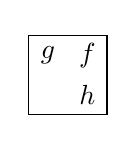
\begin{tikzpicture}[baseline=4mm]
\path (0,11mm) -- (1,1mm);
\draw (0,0) rectangle +(1,1);
\node at (.75,.25) {$h$};
\node at (.25,.75) {$g$};
\node at (.75,.75) {$f$};
\path (0,-1mm) -- (1,-1mm);
\end{tikzpicture}\,.
Figure~\ref{fig.astar2} shows the grid map after two steps of the \astar{} algorithm. Cells $(3,1)$ and $(3,0)$ receive the same cost $f$: one is closer to \p{S} (by the number of steps counted) and the other is closer to \p{G} (by the heuristics), but both have the same cost of $7$.

The algorithm needs to maintain a data structure of the \emph{open cells}, the cells that have not yet been expanded. We use the notation $(r,c,v)$, where $r$ and $c$ are the row and column of the cell and $v$ is the $f$ value of the cell. Each time an open cell is expanded, it is removed form the list and the new cells are added. The list is \emph{ordered} so that cells with the lowest values appear first; this makes it easy to decide which cell to expand next. The first three lists corresponding to Fig.~\ref{fig.astar2} are:
\begin{displaymath}
\begin{array}{l}
(4,0,5)\\
(4,1,5),\,(3,0,7)\\
(3,0,7),\,(3,1,7)\,.
\end{array}
\end{displaymath}

\begin{figure}
\subfigures
\begin{minipage}{\textwidth}
\leftfigure[c]{
\begin{tikzpicture}[scale=.8]
\pic[scale=.8] at (0,0) {astar};
\foreach \x/\y/\n in {0/0/5, 1/0/4, 0/1/6, 1/1/5, 0/2/7, 0/3/8, 1/2/6, 0/4/9, 1/3/7, 2/2/5, 3/2/4, 1/4/8, 3/3/5, 3/1/3, 3/4/6, 3/0/2, 4/1/2, 4/3/4, 4/0/1, 5/3/3, 4/4/5, 5/1/1, 5/4/4, 5/0/0}
  \node at (\x+.8,\y+.2) {\p{\n}};
\foreach \x/\y/\n in {0/0/0, 1/0/1, 0/1/1, 1/1/2, 0/2/2, 1/2/3, 2/2/4, 0/3/3, 1/3/4, 3/2/5, 3/3/6, 3/1/6}
  \node at (\x+.2,\y+.8) {\p{\n}};
\foreach \x/\y/\n in {0/0/5, 1/0/5, 0/1/7, 1/1/7, 0/2/9, 1/2/9, 2/2/9, 0/3/11, 1/3/11, 3/2/9, 3/3/11, 3/1/9}
  \node at (\x+.8,\y+.8) {\p{\n}};
\end{tikzpicture}
}
\hspace{\fill}
\rightfigure[c]{
\begin{tikzpicture}[scale=.8]
\foreach \x/\y in {0/0, 1/0, 1/1, 1/2, 2/2, 3/2, 3/1, 4/1, 5/1, 5/0}
  \draw[fill,lightgray] (\x,\y) rectangle +(1,1);
\pic[scale=.8] at (0,0) {astar};
\foreach \x/\y/\n in {0/0/5, 1/0/4, 0/1/6, 1/1/5, 0/2/7, 0/3/8, 1/2/6, 0/4/9, 1/3/7, 2/2/5, 3/2/4, 1/4/8, 3/3/5, 3/1/3, 3/4/6, 3/0/2, 4/1/2, 4/3/4, 4/0/1, 5/3/3, 4/4/5, 5/1/1, 5/4/4, 5/0/0}
  \node at (\x+.8,\y+.2) {\p{\n}};
\foreach \x/\y/\n in {0/0/0, 1/0/1, 0/1/1, 1/1/2, 0/2/2, 1/2/3, 2/2/4, 0/3/3, 1/3/4, 3/2/5, 3/3/6, 3/1/6, 3/0/7, 4/1/7, 4/0/8, 5/1/8, 5/0/9}
  \node at (\x+.2,\y+.8) {\p{\n}};
\foreach \x/\y/\n in {0/0/5, 1/0/5, 0/1/7, 1/1/7, 0/2/9, 1/2/9, 2/2/9, 0/3/11, 1/3/11, 3/2/9, 3/3/11, 3/1/9, 3/0/9, 4/1/9, 4/0/9, 5/1/9, 5/0/9}
  \node at (\x+.8,\y+.8) {\p{\n}};
\end{tikzpicture}
}
\leftcaption{The \astar{} algorithm after $6$ steps\label{fig.astar6}}
\rightcaption{The \astar{} algorithm reaches the goal cell and finds a shortest path\label{fig.astar9}}
\end{minipage}
\end{figure}

Figure~\ref{fig.astar6} shows the grid map after six steps. This can be seen by looking at the $g$ values in the upper left corner of each cell. The current list of open cells is:
\[
(3,3,9),\, (1,0,11),\, (1,1,11),\, (1,3,11)\,.
\]

The \astar{} algorithm chooses to expand cell $(3,3,9)$ with the lowest $f$. The other cells in the list have an $f$ value of $11$ and are ignored at least for now. Continuing (Fig.~\ref{fig.astar9}), the goal cell is reached with $f$ value $9$ and a shortest path in gray is displayed. The last list before reaching the goal is:
\[
(3,5,9),\, (4,4,9),\, (1,0,11),\, (1,1,11),\, (1,3,11)\,.
\]
It doesn't matter which of the nodes with value $9$ is chosen: in either case, the algorithm reaches the goal cell $(4,5,9)$.

All the cells in the upper right of the grid are not explored because cell $(1,3)$ has $f$ value $11$ and that will never be the smallest value. While Dijkstra's algorithm explored all $24$ non-obstacle cells, the \astar{} algorithm explored only $17$ cells.

\subsubsection*{A more complex example of the \astar{} algorithm}

Let apply the \astar{} algorithm to the grid map in Fig.~\ref{fig.path-sand}. Recall that this map has sand on some of its cells, so the $g$ function will give higher values for the cost of moving to these cells. The upper left diagram of Fig.~\ref{fig.a-star} shows the $g$ function as computed by Dijkstra's algorithm, while the upper right diagram shows the heuristic function $h$, the number of steps from the goal in the absence of obstacles and the sand. The rest of the figure shows four stages of the algorithm leading to the shortest path to the goal.

\begin{figure}
\begin{center}
\includegraphics[width=0.8\textwidth]{images/a-star-sand.pdf}
\end{center}
\caption{The \astar{} algorithm. Upper left: the number of steps to the goal. Upper right: the heuristic function. The middle and bottom diagrams show four steps of the algorithm.}\label{fig.a-star}
\end{figure}

Already from the middle left diagram, we see that it is not necessary to search towards the top left, because the $f$ values of the cells above and to the left of \p{S} are higher than the values to the right of and below \p{S}. In the middle right diagram, the first sand cell has a value of $13$ so the algorithm continues to expand the cells with the lower cost of $12$ to the left. In the bottom left diagram, we see that the search does not continue to the lower left of the map because the cost of $16$ is higher than the cost of $14$ once the search leaves the sand. From that point, the goal cell \p{G} is found very quickly. As in Dijkstra's algorithm, the shortest path is found by tracing back through cells with lower $g$ values until the start cell is reached.

Comparing Figs.~\ref{fig.dijkstra} and~\ref{fig.a-star} we see that the \astar{} algorithm needed to visit only 71\% of the cells visited by Dijkstra's algorithm. Although the \astar{} algorithm must perform additional work to compute the heuristic function, the reduced number of cells visited makes the algorithm more efficient. Furthermore, this heuristic function depends only on the area searched and not on the obstacles; even if the set of obstacles is changed, the heuristic function does not need to be recomputed.

\begin{framed}
\act{\astar{} algorithm}{astar}
\begin{itemize}
\item Apply the \astar{} algorithm and Dijkstra's algorithm on a small map without obstacles: place the start cell in the center of the map and the goal in an arbitrary cell. Compare the results of the two algorithms. Explain your results. Does the result depend on the position of the goal cell?
\item Define other heuristic functions and compare the results of the \astar{} algorithms on the examples in this chapter.
\end{itemize}
\end{framed}

\section{Path following and obstacle avoidance}\label{s.path-and-obstacle}
\index{path following and obstacle avoidance}

This chapter and the previous ones discussed two different but related tasks: high-level path planning and low-level obstacle avoidance. How can the two be integrated? The simplest approach is to prioritize the low-level algorithm (Fig.~\ref{fig.integrate-pp}). Obviously, it is more important to avoid hitting a pedestrian or to drive around a pothole than it is to take the shortest route to the airport. The robot is normally in its \p{drive} state, but if an obstacle is detected, it makes a transition to the \p{avoid obstacle} state. Only when the obstacle has been passed does it return to the state \p{plan path} so that the path can be recomputed.

\begin{figure}
\begin{center}
\begin{tikzpicture}[scale=.8,node distance = 2cm and 4cm,align=left,minimum size=16mm]
\node[draw,circle] (plan)  {\p{plan}\\\p{path}};
\node[draw,circle] (drive) [right=of plan] {\p{drive}};
\draw[->] (plan) to node[above,yshift=-4mm] {\p{true }$\leadsto$ \\ \p{move to goal}} (drive);
\draw[<-] (plan) to (180:15mm);
\node[draw,circle] (avoid) [below=of drive] {\p{avoid}\\\p{obstacle}};
\draw[->] (drive) to node[left,yshift=2mm] {\p{obstacle detected} $\leadsto$ \\ \p{move around obstacle}} (avoid);
\draw[->,bend left=20] (avoid) to node[left,xshift=-6mm] {\p{obstacle passed} $\leadsto$\\\p{[no action]}} (plan);
\end{tikzpicture}
\caption{Integrating path planning and obstacle avoidance}\label{fig.integrate-pp}
\end{center}
\end{figure}

The strategy for integrating the two algorithms depends on the environment. Repairing a road might take several weeks so it makes sense to add the obstacle to the map. The path planning algorithm will take the obstacle into account and the resulting path is likely to be better than one that is changed at the last minute by an obstacle avoidance algorithm. At the other extreme, if there are a lot of moving obstacles such as pedestrians crossing a street, the obstacle avoidance behavior could be simply to stop moving and wait until the obstacles move away. Then the original plan can simply be resuming without detours.

\begin{framed}
\act{Combining path planning and obstacle avoidance}{combi}
\begin{itemize}
\item Modify your implementation of the line-following algorithm so that the robot behaves correctly even if an obstacle is placed on the line. Try several of the approaches listed in this section.
\item Modify your implementation of the line-following algorithm so that the robot behaves correctly even if additional robots are moving randomly in the area of the line. Ensure that the robots do not bump into each other.
\end{itemize}
\end{framed}

\section{Summary}

Path planning is a high-level behavior of a mobile robot: finding the shortest path from a start location to a goal location in the environment. Path planning is based upon a map showing obstacles. Dijkstra's algorithm expands the shortest path to any cell encountered so far. The \astar{} algorithm reduces the number of cells visited by using a heuristic function that indicates the direction to the goal cell.

Path planning is based on a graph such as a grid map, but it can also be done on a continuous map by creating a graph of obstacles from the map. The algorithms can take into account variables costs for visiting each cell.

Low-level obstacle avoidance must be integrated into high-level path planning.

\section{Further reading}

Dijkstra's algorithm is presented in all textbooks on data structures and algorithms, for example, \cite[Sect.~24.3]{crls3}. Search algorithms such as the \astar{} algorithm are a central topic of artificial intelligence \cite[Sect.~3.5]{ai}.

\bibliographystyle{spmpsci}
\bibliography{er}
